\section{Method}

An image $f(u,v)$ can be representet using an illumination-reflection model. 
\begin{figure}[h!]
\begin{equation}
  f(u,v) = i(u,v) r(u,v)
  \label{eqn:im1}
\end{equation}
\caption{image $f$ represented with an illumination component $i$ and reflection component $r$}
\end{figure}
The illumination $i(u,v)$ can be charectarize as slow changes in the frequency domain or as glooming light in the spartial domain. While the reflection $r(u,v)$ tends to be rapid changes in the frequenze domain or as edges in the spartial domain. The homomorphic filter works in the frequenzy domain and aims to filter out some of the illumination $i(u,v)$. This results in an incresment in contrast and normalized brightness. \\

\subsection{Pre-poccesing of the original image}
To apply the filter the image $f(u,v)$ needs to be transformed into frequenzy domain and since the illumination-reflection model is multiplicativ and will result in a convulotion in frequency space the image will need to be pre-proccesed before the transformation.

\begin{figure}[h!]
\begin{equation}
  \mathfrak{F}[f(u,v)] = \mathfrak{F}[i(u,v)] \ast \mathfrak{F}[r(u,v)] 
  \label{eqn:transWithoutLogRes}
\end{equation}
\begin{equation}
  \mathfrak{F}[f(u,v)] \neq \mathfrak{F}[i(u,v)] \mathfrak{F}[r(u,v)] 
  \label{eqn:transWithoutLogErr}
\end{equation}
\caption{Multiplication will become convulotion (\ref{eqn:transWithoutLogRes}) in frequency domain and not remain a multiplication.(\ref{eqn:transWithoutLogErr})}
\end{figure}

Applying the logarimic transformation on the original image results in a transformation of the illumination-reflection model from multiplicativ to additive, Eq \ref{eqn:log}. The Fourier transform is applied to the resulting image of the logaritmic transform and the illumination/reflection model is intact and in frequenzy domain, since additon remains as addition in fourier transformation.
\begin{figure}[h!]
\begin{equation}
  f(u,v) = i(u,v) r(u,v) \xrightarrow{\ln} \ln{f(u,v)} = \ln{i(u,v)} + \ln{r(u,v)} 
  \label{eqn:loga}
\end{equation}
  \begin{equation}
    \begin{split}
      Z(u,v) &= \mathfrak{F} [\ln{f(u,v)}]\\ &= \mathfrak{F}[\ln{i(u,v)}] + \mathfrak{F}[\ln{r(u,v)}]\\ &= F_i(u,v) + F_r(u,v)
    \end{split}
    \label{eqn:logtrans}
  \end{equation}
\caption{image $f$ represented with an illumination component $i$ and reflection component $r$, in Eq \ref{eqn:loga} multiplication becomes additiv after logarithmic transform. Eq \ref{eqn:logtrans} shows the Fouriered and logarithmic transformed image $Z$ and it's illumination and reflection component. }
\end{figure}

Since the images are discrete, the Fourier Transform the image will loop the image periodically. To avoid aliasing the source image is zero padded. Zero Padding the source image using matlabs \textit{padarray}- function. The amount of zeros padded with the image is calculated using equations \ref{eqn:Ppadded} and \ref{eqn:Qpadded} given in the coursebook\cite[p. 274]{dipBook}. Exempel of zeropadding is shown in Figure \ref{fig:zeropadded}.
\begin{figure}[h!]
\begin{equation}
  P \geq 2M -1
  \label{eqn:Ppadded}
\end{equation}
\caption{4.6-31, P Resulting horisontal size of the image, M horizontal size of source image}
\end{figure}

\begin{figure}[h!]
  \begin{equation}
    Q \geq 2N -1
    \label{eqn:Qpadded}
  \end{equation}
  \caption{4.6-31, Q Resulting horisontal size of the image, N horizontal size of source image}
\end{figure}

\begin{figure}[h!]
  \begin{center}
    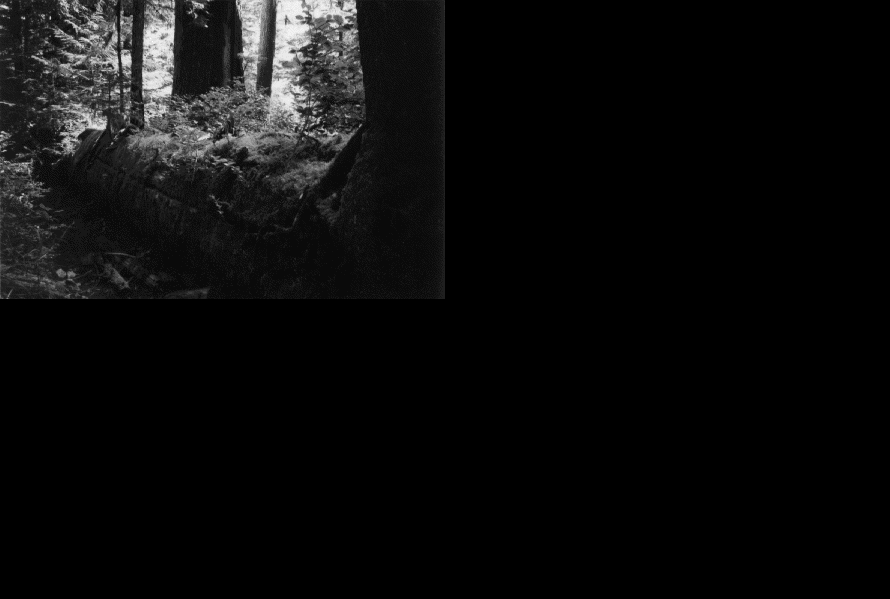
\includegraphics[width=0.6\textwidth]{pics/zeroPadded.png}
  \end{center}
  \caption{Original image padded with P-M and Q-N zeros after original matrix using \textit{padarray} in matlab.}
  \label{fig:zeropadded}    
\end{figure}

The filter used in this project is center positioned. Since matlabs \textit{fft2}-function returns the transformed image with the origio in upper left corner, the result must be shifted to apply the filter correctly. Shifting the transformation is done using matlabs \textit{fftshift}.

\subsection{The construction of the homomorphic filter}
The filter used to enhanced the image in this paper is a highpass guassian filter,Eq \ref{eqn:gaussian_filter}, with three parametes. 
    \begin{equation}
    \label{eqn:gaussian_filter}
      H(u,v) = \left( \gamma_H - \gamma_L \right) \left[ 1 - e^{- D(u,v) /2 * D_0^2}\right] + \gamma_L 
    \end{equation}

\begin{itemize}
  \item $\gamma_H$ wich sets the maximum amplitude of the filter.\\
  \item $\gamma_L$ wich sets the lower bound of amplitude of the filter.\\
  \item $D_0$ is sets the cut-of freqenzy, to control the stepness and width of the guassian function.
  \item $D(u,v)$ is a function to calculate the distance from the center of the filter to each element ,$u,v$, in the filter. 
\end{itemize}

\begin{figure}[h!]
  \begin{lstlisting}
    [u, v] = meshgrid(1:q,1:p);
    centerU = ceil(q/2);
    centerV = ceil(p/2);
    gaussianNumerator = ((u - centerU).^2 + (v - centerV).^2);
  \end{lstlisting}
  \label{code:raduv}
  \caption{Matlab code of the distance function $D(u,v)$ used in the filter. p and q is the size of the image after zeropadding.}
\end{figure}

\subsection{Applying the filter and the post processing}

The filter is applied by multiplication in the Frequency domain as seen in Figure \ref{fig:filteringOfImage}. 
\begin{figure}[h!]
  \begin{equation}
    S(u,v) = Z(u,v)H(u,v)
    \label{eqn:applyfilt}
  \end{equation}
  \caption{S: the filtered image, Z: pre-processed image from Eq \ref{eqn:logtrans}, H: highpass guassian filter described in Eq \ref{eqn:gaussian_filter} }
  \label{fig:filteringOfImage}    
\end{figure}

Post processing consists of four steps. Shifting the filtered image to get the origo in top/left corner. Apply the inverset fourier transform. Crop the zero padding to obtain the original image dimensions. Inverse logarithm transformation by taking the exponential function of the result of croped image. The result of the post process is homomorphic filtered image.